\section{Time Planning}

Overall the project was timed reasonably well, every deliverable was completed to the expected quality by the required deadline. The specification was revised with the customer prior to finalisation, the poster was delivered on time despite issues with the printing contractor, the final resort and the software deliverable were also completed and delivered on time. The only time management issues were related to soft deadlines which were internal to the project and had no impact on the project.

\paragraph{Issues with time tanagement}
The project was scheduled to take advantage of the time mutually available in term one, and avoid infringing study time for other modules in term 2 and 3. 
%% REF STAGEGATE from spec?
By the end of the first term the project should have been at the alpha stage, but the volume of the work required was drastically underestimated, as was the number of work hours available. It was important to ensure the group spent a lot of time together to avoid miscommunications and to ease collaborative efforts, so a lot of effort went into scheduling coding session each week and emergency development weekends to mitigate any delays that occurred. The term 2 scheduling focused mainly on fixing minor bugs, strengthening weak points and developing advanced features beyond the project's requirements, but upon reflection, many of the features scheduled for completion in term 1 bled over all the way to the end of term 2. 

\begin{figure*}
	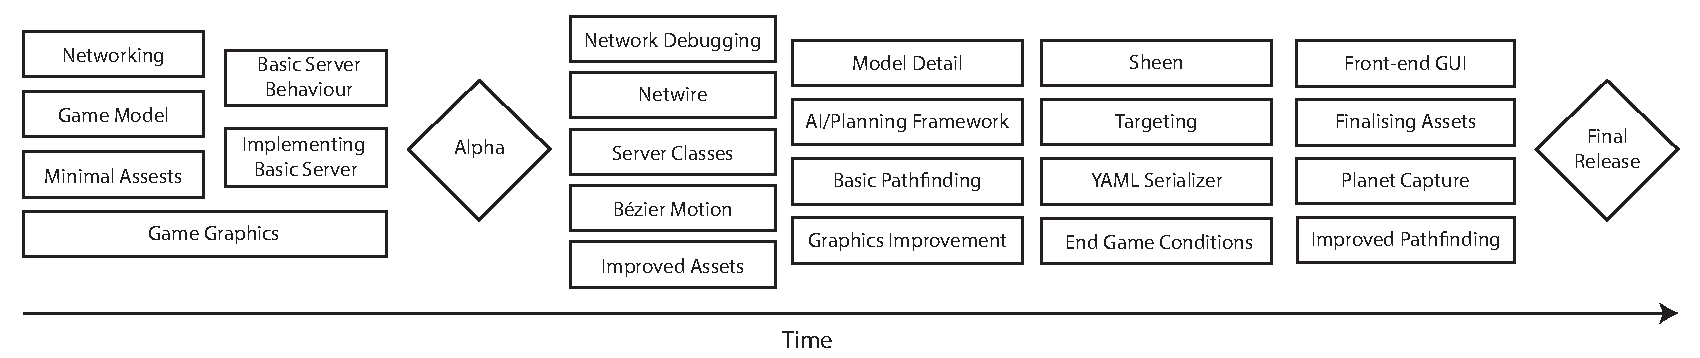
\includegraphics[height=33em]{res/pm/actual_workflow_diagram}
	\label{fig:actual_workflow_diagram}
	\caption{Actual workflow of project}
\end{figure*}

Casual conversation was issue throughout the course of the project, very often a concise meeting deteriorated into off-topic conversation and cost the project valuable time, the informal atmosphere in the project group exasperated the problem since the management roles couldn't failed as a part-time occupation, and there was no ``bad guy'' to keep the group focused on project work all the time.

Not only was it difficult to maintain a good working pace, but it became difficult to assess the appropriate amount of time to ask of each team member since the number of university contact hours per week fluctuated as modules began/ended and as other assignments were set.

\paragraph{Unavoidable issues}
One of the earliest issues arising with the schedule was attempting to arrange collaboration sessions which didn't conflict with any group member's other arrangements (particularly university assignments and contact hours). Rather than working asynchronously, the group decided to meet later in the evening and on weekends, when group members were tired and less productive, this meant the working hours became less and less productive, making milestones harder to reach on schedule as the project progressed.

An unavoidable issue in most projects is what's known as student syndrome, where people only start to fully apply themselves to a task in the last possible moment before a deadline.
%% CITE PROJECT MANAGEMENT BOOK
Although lack of motivation was never a problem, it was often the case that the team spent too much time perfecting something that is already of an acceptable quality, when there are other project components which desperately need work.

The most severe problem was having a slight underestimate of the time required for each project component. It's very difficult to accurately gauge how much work will be required to complete a particular task, and the schedule is almost always an underestimate. Even under the most efficient working conditions, the project gradually slipped further and further behind schedule until many unfinished components were under threat of being unfinished by the delivery date.

\paragraph{Conclusions drawn from time tanagement}
The initial scheduling of the project was overambitious, and it took quite a few emergency work sessions to bring the project back on schedule. Time could have been managed more effectively if the estimates were more realistic, however, an overestimate of time might have made the project team more prone to the aforementioned student syndrome, lower efficiency. Time estimation can is a double edged sword, since it takes a delicate balance to not damage the progress of the project by underestimating or overestimating, but in practice it's impossible to accurately predict how much time a certain tasks will take since the time required for debugging varies massively between bugs. 

The problem with scheduling in software projects is that any time allocated for fixing unknown bugs and fine tuning features can be used as a means for a developer to defer fixing detected bugs because they can be dealt with later, the problem being is that deferred bugs will then cost the project even more time because important issues weren't dealt with at the time, so not only will there be a context switching overhead for any deferred bugs, there may be extremely serious, yet undetected bugs that then cost the developers debugging time which hasn't been accounted for in the project schedule. One possible solution to such delays is to keep the entire team motivated to meet soft deadlines throughout the project so the team is kept forced to deal with delays promptly, that way the effect of delays for the overall project is largely mitigated. 
%tcq res 
% http://www.leonelson.com/wp-content/uploads/2005/04/projecttriangle.gif

